\documentclass[11pt,letterpaper]{article}
\usepackage{tikz}
\usetikzlibrary{calc,patterns,decorations.pathmorphing,decorations.markings}
\topmargin 0in
\oddsidemargin 0in
\evensidemargin 0in
\headheight 0in
\headsep 0in
\topskip 0in
\textheight 9in
\textwidth 6.5in

\begin{document}
  \title{Simple Harmonic Motion}
  \author{Bob Forcha}
  \date{\today}
  \maketitle

  \tableofcontents

  \section{Overview}
  Simple harmonic motion (SHM) is the term used to describe the motion
  of a mass connected to a spring, as shown below.\\

  \begin{center}
    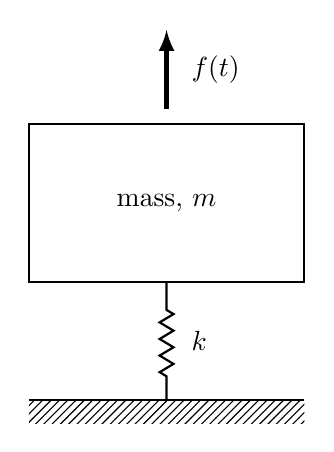
\begin{tikzpicture}[every node/.style={draw,outer sep=0pt,thick}]
      \tikzstyle{spring}=[thick,decorate,decoration={zigzag, pre length=0.3cm,post length=0.3cm,segment length=6}]
      \tikzstyle{ground}=[fill,pattern=north east lines,draw=none,minimum width=0.75cm,minimum height=0.3cm]
      
      \node (M) [minimum width=3.5cm,minimum height=2cm] {mass, $m$};

      \node (ground1) at (M.south) [ground,yshift=-1.5cm,anchor=north,minimum width=3.5cm] {};
      \draw (ground1.north west) -- (ground1.north east);
      \draw [spring] (ground1.north) -- (M.south) node[midway,right,xshift=0.2cm,draw=none] {$k$};
      \draw [-latex,ultra thick] (M.north) ++(0,0.2cm) -- +(0,1cm) node[midway,right,xshift=0.2cm,draw=none] {$f(t)$};
    \end{tikzpicture}
  \end{center}
    
  Let's take a look at the free body diagram for this one-dimensional system:\\

  \begin{center}
    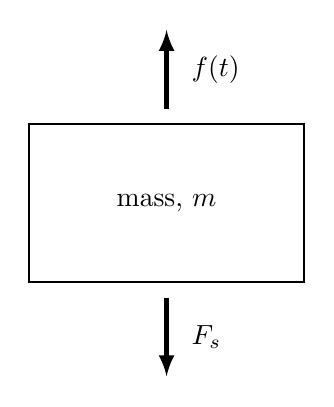
\begin{tikzpicture}[every node/.style={draw,outer sep=0pt,thick}]
      \node (M) [minimum width=3.5cm,minimum height=2cm] {mass, $m$};
      \draw [-latex,ultra thick] (M.north) ++(0,0.2cm) -- +(0,1cm) node[midway,right,xshift=0.2cm,draw=none] {$f(t)$};
      \draw [-latex,ultra thick] (M.south) ++(0,-0.2cm) -- +(0,-1cm) node[midway,right,xshift=0.2cm,draw=none] {$F_s$};
    \end{tikzpicture}
  \end{center}

  From here we can write the equation of motion:\\

  $$\Sigma F_{x} = m\ddot{x} = f(t) - F_{s}$$

  Hook's Law tells us that for a spring, the force required to
  strech it is proportional to the length it is being stretched,
  or $F_s = kx$, yielding

  $$m\ddot{x} = f(t) - kx$$
  $$m\ddot{x} + kx = f(t)$$

  Let's assume the simplest $f(t)$ possible, $f = 0$:

  $$m\ddot{x} = -kx$$
  $$\Rightarrow \ddot{x} = \frac{k}{m}x$$
  $$\Rightarrow x(t) = A\sin\left(\sqrt{\frac{k}{m}}t\right) + B\cos\left(\sqrt{\frac{k}{m}}t\right)$$

  Figuring out the coefficients:

  $$x(0) = x_0 = A\sin\left(0\right) + B\cos\left(0\right)$$
  $$\Rightarrow x_0 = B$$
  $$\Rightarrow x(t) = A\sin\left(\sqrt{\frac{k}{m}}t\right) + x_{0}\cos\left(\sqrt{\frac{k}{m}}t\right)$$
  $$\dot{x} = A\sqrt{\frac{k}{m}}\cos\left(\sqrt{\frac{k}{m}}t\right) - x_{0}\sqrt{\frac{k}{m}}\sin\left(\sqrt{\frac{k}{m}}t\right)$$
  $$\Rightarrow \dot{x}(0) = \dot{x_0} = A\sqrt{\frac{k}{m}}\cos\left(0\right) - x_{0}\sqrt{\frac{k}{m}}\sin\left(0\right)$$
  $$\Rightarrow \dot{x_0}\sqrt{\frac{m}{k}} = A$$
  $$\Rightarrow x(t) = \dot{x_0}\sqrt{\frac{m}{k}}\sin\left(\sqrt{\frac{k}{m}}t\right) + x_{0}\cos\left(\sqrt{\frac{k}{m}}t\right)$$

\end{document}